\clearpage
\myparagraph{\olly}
\myindex{\olly}

Let's load this example into \olly. 
Let the input value be \TT{0x12345678}.

For $i=1$, we see how $i$ is loaded into \ECX: 

\begin{figure}[H]
\centering
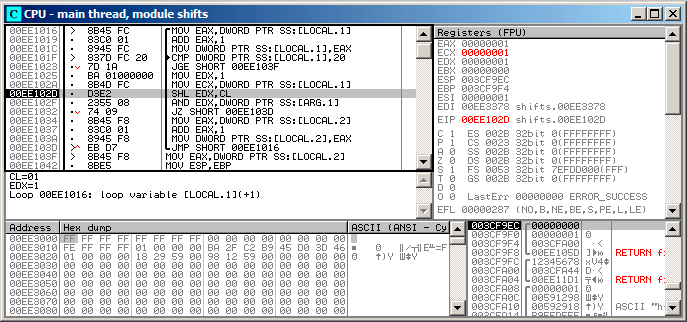
\includegraphics[scale=\FigScale]{patterns/14_bitfields/4_popcnt/olly1_1.png}
\caption{\olly: $i=1$, $i$ is loaded into \ECX}
\label{fig:shifts_olly1_1}
\end{figure}

\EDX is 1. \SHL is to be executed now.

\clearpage
\SHL was executed:

\begin{figure}[H]
\centering
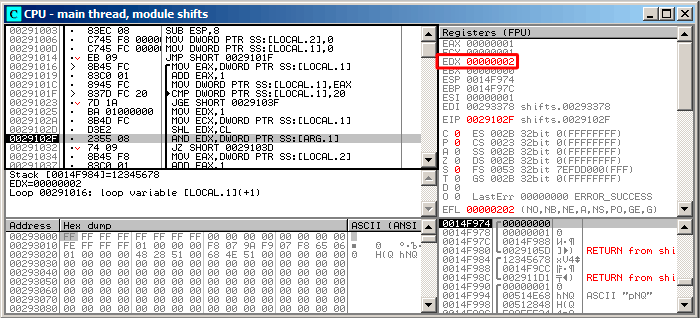
\includegraphics[scale=\FigScale]{patterns/14_bitfields/4_popcnt/olly1_2.png}
\caption{\olly: $i=1$, \EDX=$1 \ll 1=2$}
\label{fig:shifts_olly1_2}
\end{figure}

\EDX contain $1 \ll 1$ (or 2). This is a bit mask.

\clearpage
\AND sets \ZF to 1, which implies that the input value (\TT{0x12345678})  ANDed with 2 results in 0:

\begin{figure}[H]
\centering
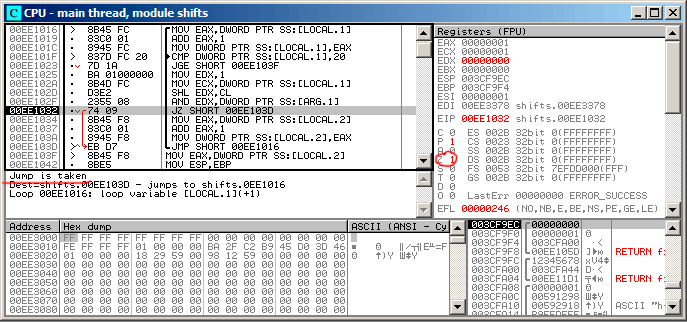
\includegraphics[scale=\FigScale]{patterns/14_bitfields/4_popcnt/olly1_3.png}
\caption{\olly: $i=1$, 
is there that bit in the input value? No. (\ZF=1)}
\label{fig:shifts_olly1_3}
\end{figure}

So, there is no corresponding bit in the input value.

The piece of code, which \glslink{increment}{increments} the counter is not to be executed: 
the \JZ instruction \emph{bypassing} it.

\clearpage
Let's trace a bit further and $i$ is now 4.
\SHL is to be executed now:

\begin{figure}[H]
\centering
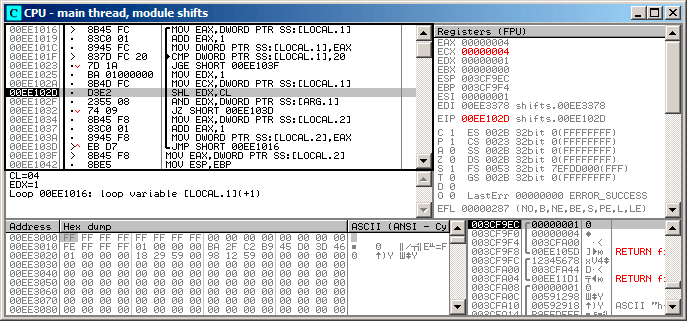
\includegraphics[scale=\FigScale]{patterns/14_bitfields/4_popcnt/olly4_1.png}
\caption{\olly: $i=4$, $i$ is loaded into \ECX}
\label{fig:shifts_olly4_1}
\end{figure}

\clearpage
\EDX=$1 \ll 4$ (or \TT{0x10} or 16): 

\begin{figure}[H]
\centering
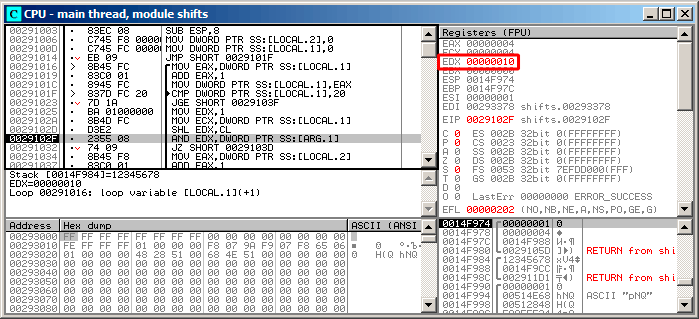
\includegraphics[scale=\FigScale]{patterns/14_bitfields/4_popcnt/olly4_2.png}
\caption{\olly: $i=4$, \EDX=$1 \ll 4=0x10$}
\label{fig:shifts_olly4_2}
\end{figure}

This is another bit mask.

\clearpage
\AND is executed:

\begin{figure}[H]
\centering
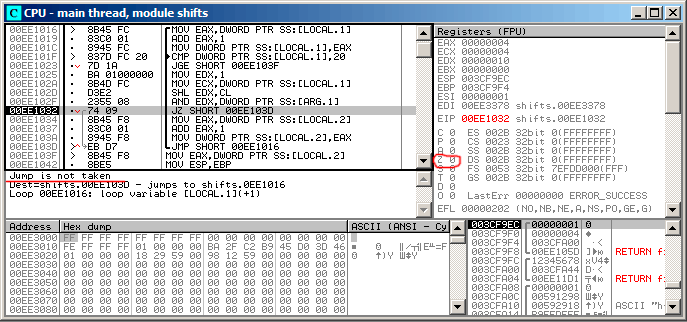
\includegraphics[scale=\FigScale]{patterns/14_bitfields/4_popcnt/olly4_3.png}
\caption{\olly: $i=4$, 
is there that bit in the input value? Yes. (\ZF=0)}
\label{fig:shifts_olly4_3}
\end{figure}

\ZF is 0 because this bit is present in the input value.
Indeed, \TT{0x12345678 \& 0x10 = 0x10}. 

This bit counts: the jump is not triggering and the bit counter 
\glslink{increment}{incrementing}.

The function returns 13. 
This is total number of bits set in \TT{0x12345678}.

